\chapter{Asking Miami Moguls How They Got Rich!}

This lecture is not a blackboard lecture, but it does have a mathematical spine. The mathematics comes to us in the form of growth rates, return calculations, budget constraints, debt coverage, and threshold conditions for what several speakers call financial freedom. We begin with wealth as spectacle, then rewind into a more interesting problem: how a city full of visible luxury might be read as a laboratory of systems, cash flow, risk, and accumulated assets.

\section{Miami as a Search Field for Wealth}

The lecture opens with a teaser, but its true beginning comes a moment later when the trip is framed explicitly. The host tells us that Miami now has substantially more millionaires than it did a decade ago, and that he intends to treat the city as a field in which hidden wealth may be found and interrogated. That statistic is not derived inside the lecture, but it gives the inquiry a quantitative edge:

\begin{equation}
M_{\mathrm{Miami,now}} \approx 1.75\,M_{\mathrm{Miami,10y}}.
\end{equation}

We should be careful here. This is not yet a theorem about wealth creation; it is a framing device. But it matters because the lecture is thereby converted from a montage of luxury into a search problem. We are not merely looking at expensive stores and expensive cars. We are asking what operating rules, if any, can be extracted from the people who move through such a place.

The host's motivating question is also stated with unusual clarity. He wants to know how these people got to where they are, and how an ordinary viewer might begin a path toward financial freedom. So even at the outset the lecture has two levels: visible wealth above, mechanism below.

\section{Street Filtering, Persistence, and the First Loud Case}

Once the lecture reaches the Design District, it refuses to proceed cleanly. There are refusals, awkward encounters, partial recognitions, and social friction. This is not filler. It is part of the substance. Access to high-net-worth operators is itself scarce, and the repeated ``come on'' cadence in the lecture keeps reminding us that the inquiry advances by persistence rather than by tidy classroom sequencing.

The first major interview is Johnny, and the tone changes immediately. He reports very large business outcomes, beginning with a year above one hundred million dollars and then, later in the exchange, annual business in the neighborhood of one hundred fifty to one hundred seventy million dollars. The lecture also preserves the much larger lifetime business claim:

\begin{align}
R_{\mathrm{Johnny},2021} &> \$100\,\mathrm{M},\\
R_{\mathrm{Johnny,annual}} &\in [\$150\,\mathrm{M},\,\$170\,\mathrm{M}],\\
S_{\mathrm{career}} &> \$2\,\mathrm{B}.
\end{align}

These numbers should be treated as reported claims, not audited statements. Their role in the lecture is evidentiary rather than statistical: they justify why the host keeps pressing.

\paragraph{Mechanism.} Johnny's first principle is not accounting but psychology. He says that success in sales depends on understanding human nature and not pushing people too hard. This is not formalized, but the lecture uses it as an opening move: before capital, before systems, there is perception.

\paragraph{Risk.} He also insists that he funded himself, and that once he reached scale, banks began to seek him out rather than the other way around. Here the causal picture is rough but recognizable: first self-finance, then success, then leverage on much better terms.

\subsection{Question \& Answer: What Do We Do About a Bad Month?}

The lecture raises this question directly because it is the natural objection to every large revenue claim. If the upside is real, what happens on the downside?

Johnny's answer is not a model of cyclicality. It is almost the opposite. He says that he could never understand the idea of a bad month, and that after a certain point in his career he had not had one. We should not smooth this into a general theory. The point of the answer is temperamental and strategic: once an operator has product-market force, opportunity, and preparation aligned, his lived experience of volatility changes.

A concise way to preserve the lecture's logic is to keep the slogan he later supplies:
\begin{equation}
\text{opportunity} + \text{preparation} \longrightarrow \text{luck}.
\end{equation}

This is not an identity in any strict sense, but it is the lecture's way of reinterpreting luck as an event that occurs when prior readiness meets a live opening.

The host closes this episode by calling it one of the wildest interactions on the channel. That recap matters. It gives us a pause before the lecture moves from flamboyant wealth talk to a more disciplined account of operations.

\section{Hospitality, Honesty, and the Refusal of Final Freedom}

The next substantial interview comes from the restaurant world, and the lecture deliberately changes register. Here the mechanism of wealth is not presented as raw aggression or verbal force. It is presented as service, hospitality, team quality, honesty with friends and investors, and a great deal of hard work.

We should preserve the contrast. The lecture is not saying that one wealth style refutes the other. It is saying that Miami contains multiple operating logics, and the chapter must not flatten them into a single entrepreneur template.

The most interesting conceptual turn in this segment comes when the host asks about the turning point to financial freedom. Instead of affirming the phrase, the restaurant owner resists it. There is, in his telling, no permanent resting state. One keeps working harder, keeps pushing, keeps extending the enterprise.

\begin{remark}
The phrase ``financial freedom'' is unstable in this lecture. Anthony Powell and Eric Spofford will treat it as a threshold condition. The Poppy Steak interview, by contrast, treats it as a misleading endpoint. We should keep that tension alive rather than forcing agreement.
\end{remark}

So this section functions as a corrective. Wealth is not only a matter of dramatic exits, extraordinary product placement, or high-stakes risk. It is also the slow discipline of service quality, team quality, and partner honesty.

\section{The Gym-Business Failure Model}

The gym entrepreneur enters first as a story of self-belief. He describes immigrant background, scarcity, improvisation, relentless advertising, and a refusal to accept ``no.'' But the lecture does not leave the matter at inspiration. It pivots into something much sharper: a failure model.

He reports a rough survival statistic and then gives a concrete reason why many ventures die before they ever open. The problem is not abstract lack of motivation. It is cost structure. The startup budget is too small relative to the fixed burdens being assumed.

The lecture gives us three numerical anchors:

\begin{align}
B_{0,\mathrm{gym}} &\approx \$500{,}000,\\
E_{\mathrm{gym}} &\in [\$300{,}000,\$500{,}000],\\
L_{m,\mathrm{gym}} &= \$38{,}000/\mathrm{month}.
\end{align}

Already one sees the shape of the argument. If equipment spending consumes most of the initial budget, and the location comes with a very heavy monthly lease, then the venture is fragile before the first stable stream of revenue has arrived.

\subsection{Question \& Answer: Why Do Businesses Die Before They Open?}

The lecture poses this as a practical puzzle, and the answer is not mysterious.

\begin{enumerate}
\item The entrepreneur begins with an initial budget \(B_{0,\mathrm{gym}}\) that looks large in isolation.
\item A very large portion of that budget is committed immediately to equipment, \(E_{\mathrm{gym}}\).
\item The lease burden is then layered on top of that commitment at \(L_{m,\mathrm{gym}}=\$38{,}000\) per month.
\item If the owner also assumes payroll, carrying costs, and other reserves, the margin for error becomes tiny.
\item The business is therefore under stress before it has had time to stabilize operations or member acquisition.
\end{enumerate}

A simple numerical check helps us see why the lecture insists on this point. One year of rent at the quoted figure is

\begin{equation}
12L_{m,\mathrm{gym}} = 12 \times \$38{,}000 = \$456{,}000.
\end{equation}

This does \emph{not} mean that one prepays a full year of rent at launch. The point is different: the annualized fixed burden is already of the same order as the total startup budget being discussed. Once we place that beside equipment expense, the lecture's warning becomes legible. The failure is often built into the initial structure.

So the real lesson here is not ``work hard'' in the abstract. It is that fixed obligations can consume a business before the owner has created enough operational slack to survive.

\section{Interlude: Side Hustles and Income Architecture}

At this point the lecture breaks its interview rhythm and inserts a sponsor-driven remark: forty-five percent of millionaires in the United States have a side hustle. We should preserve this carefully and lightly. It is a host-stated statistic, not a result proven by the lecture.

Still, it serves a structural purpose. The lecture is moving away from isolated stories and toward a broader architecture of income. The implication is that wealthy households often do not rely on a single stream. They build layers.

This interlude is therefore best treated not as a theorem but as a bridge. It prepares us for Anthony Powell, where the lecture becomes much more explicit about allocation, compounding, and the difference between earned income and asset-generated income.

\section{Anthony Powell: System, Earned Income, and the 8-Plex}

Anthony Powell provides the cleanest formal sequence in the lecture. He begins in the language of systems. McDonald's is his first example, not because of cuisine, but because a good system can be run repeatedly and predictably. He claims to have built such systems in direct sales, contact management, and lead distribution.

Then the lecture pivots from system in business to system in money.

\paragraph{Step 1.} Find a vehicle that produces substantial earned income.

\paragraph{Step 2.} Do not spend that earned income.

\paragraph{Step 3.} Invest it in assets.

A compact mathematical rendering of this sequence is

\begin{align}
S_t &= Y_{e,t} - C_t,\\
A_{t+1} &= A_t + S_t,
\end{align}

where \(Y_{e,t}\) is earned income, \(C_t\) is consumption, \(S_t\) is investable surplus, and \(A_t\) is the asset base. The lecture's phrasing is informal, but the structure is unmistakable.

\subsection{Question \& Answer: What Do We Do With the First \$10{,}000 or \$20{,}000?}

Anthony poses the practical objection himself: everyone has heard ``buy assets,'' but where does one actually begin? His first answer is the S\&P ETF.

The lecture gives a worked example. If one has \$100{,}000 invested and the market is up \(17\%\), then the gain is

\begin{align}
\Delta V &= rV_0,\\
\Delta V &= 0.17 \times \$100{,}000 = \$17{,}000,\\
V_1 &= V_0 + \Delta V = \$117{,}000.
\end{align}

This is elementary arithmetic, but it matters because it is one of the few places where the lecture slows down enough for us to see the mechanism. The point is not merely that markets go up. The point is that once capital is placed into an asset, wealth can move without requiring a matching increment of personal labor at that moment.

Anthony then adds the regular-deposit rule. One contributes what one can---\$250, \$500, \$1{,}000 a month---and lets the asset base accumulate while one continues to work aggressively in the active-income vehicle.

\subsection{Question \& Answer: How Can an 8-Plex Pay for Itself?}

The lecture's strongest quasi-mathematical example is the 8-plex. Anthony says that when he was broke he needed his rent paid, so he bought an eight-unit multifamily property. The bank, in his account, is willing to lend because the property can be judged by cash flow.

We may formalize his spoken logic cautiously. Let
\[
n=8,\qquad n_{\mathrm{paying}}=7,
\]
where one unit is treated as the owner's effective position and seven are rent-paying units. Let \(c_u\) be the average monthly net contribution of one paying unit toward debt service, and let \(D_m\) denote the monthly debt load. The lecture's condition is then

\begin{equation}
7c_u \ge D_m.
\end{equation}

If that inequality holds, then the seven paying units cover the debt burden, and the owner's position is, in his rhetoric, ``free.'' We should keep his phrase but interpret it carefully: not literally free, but effectively absorbed by the cash flow of the property.

\begin{figure}[h]
\centering
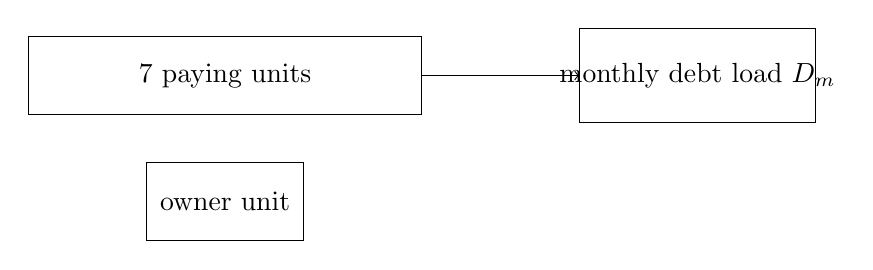
\begin{tikzpicture}[x=1cm,y=1cm]
\draw (0,0) rectangle (5,1);
\node at (2.5,0.5) {7 paying units};

\draw (1.5,-1.6) rectangle (3.5,-0.6);
\node at (2.5,-1.1) {owner unit};

\draw[->] (5,0.5) -- (7,0.5);
\draw (7,-0.1) rectangle (10,1.1);
\node at (8.5,0.5) {monthly debt load \(D_m\)};
\end{tikzpicture}
\caption{Transcript-derived schematic of the 8-plex argument. The lecture's claim is that seven paying units can cover the monthly debt load, leaving the owner's position effectively carried by property cash flow.}
\end{figure}

From there the lecture adds the value-add step: improve the property, increase value, sell, and double the money. We should not pretend that a complete return model has been supplied. The lecture gives no cap rate, no vacancy rate, no financing schedule, and no tax treatment. But it does give the narrative sequence, and that sequence is central:
\[
\text{earned income} \longrightarrow \text{asset purchase} \longrightarrow \text{cash flow} \longrightarrow \text{value increase} \longrightarrow \text{liquidity event}.
\]

Anthony closes this section with a hard distinction: he does not spend earned income. The lecture wants us to hear this as a rule of class migration. Work produces income; assets purchase freedom.

\section{Eric Spofford: Section 8, Cash Flow, and the Threshold of Freedom}

The Eric Spofford interview begins with a different kind of credential. Not only a large exit, but also a recovery narrative. He presents himself as someone who took a deeply personal transformation and turned it into a niche business that eventually sold for over one hundred million dollars.

Then he answers the lecture's next financial question in a way that is more accessible than the yacht setting would suggest. His recommendation is Section~8 real estate. The transcript becomes partially garbled in this portion, so we must be careful. But several claims come through clearly: the average price per property is said to be below \$100{,}000, the asset class is presented as accessible to ordinary Americans, and the cash-on-cash return is said to be supported by government overpayment of rent in order to stimulate low-income housing supply.

The entry-price claim may be recorded as

\begin{equation}
P_{\mathrm{Section8,avg}} < \$100{,}000.
\end{equation}

Again, we preserve this as a speaker's claim, not an external market survey.

\begin{definition}
In the Anthony--Eric sense of the lecture, financial freedom is reached when passive asset income covers lifestyle cost:
\begin{equation}
I_p \ge C_l.
\end{equation}
Here \(I_p\) denotes passive cash flow from assets, and \(C_l\) denotes the ongoing cost of the lifestyle one intends to support.
\end{definition}

This definition captures the strongest mathematical compression in the lecture. One saves from earned income, acquires appreciating cash-flowing assets, and repeats until the flow from assets can fund life directly.

\subsection{Question \& Answer: How Can an Ordinary American Become Financially Free?}

Eric's answer proceeds in an ordered way even though it is spoken rather than written.

\begin{enumerate}
\item Reduce lifestyle consumption somewhat.
\item Save from earned income rather than spending it all.
\item Put savings into appreciating, cash-flowing assets.
\item Continue until the stream of passive cash flow is large enough to carry the desired lifestyle.
\item At that point, work becomes optional in a strong sense: one acts because one wants to, not because one must.
\end{enumerate}

This is the lecture's cleanest threshold argument, and it belongs near the end because it gathers together the whole prior sequence: city-level wealth concentration, street-level access, entrepreneurial earnings, budgeting discipline, asset accumulation, and then freedom through cash flow rather than through display.

Eric's final compression is moral as much as financial. Avoid vice. Choose one's circle carefully. Be loyal to one's future. The lecture is not content with a balance-sheet story alone. It wants character, environment, and incentives to appear in the same frame as returns and rent.

\section{Summary}

The lecture begins with luxury as evidence and ends with assets as mechanism. Along the way it gives us several distinct wealth logics: Johnny's psychology, risk, and self-financing; the restaurateur's service, honesty, and refusal of any final resting point; the gym entrepreneur's warning about destructive startup structure; Anthony Powell's progression from earned income to assets; and Eric Spofford's threshold view of financial freedom.

The mathematics is simple but decisive. A city can be described by growth in its millionaire count. A market gain can be described by \(\Delta V=rV_0\). A property can be judged by whether tenant cash flow covers debt load. A life can be judged, in one important sense, by whether passive income exceeds lifestyle cost. The lecture's deepest claim is that wealth becomes durable not at the moment of display, but at the moment when the structure underneath begins to carry itself.